\documentclass[./main.tex]{subfiles}
\graphicspath{{\subfix{./Abbildungen/}}}

\begin{document}
\renewcommand{\tasktitle}{Test OC Synthese}
\renewcommand{\taskpoints}{5}
\renewcommand{\taskweight}{7.9}
\aufgabenanfang
\blindtext

\kasten{5cm}{
    Antwort\punkte{5}
}{}

% \begin{center}    
% \begin{tabular}{ccc}
%     \begin{minipage}[c]{3cm}
%         \kasten{2cm}{\textbf{A}\par\begin{center}abc\end{center}}{}
%     \end{minipage} &
%     \begin{minipage}[c]{3cm}
%         \kasten{2cm}{\textbf{B}\\def}{}
%     \end{minipage}&
%     \begin{minipage}[c]{3cm}
%         \kasten{2cm}{\textbf{C}\\ghi}{}
%     \end{minipage}\\
% \end{tabular}
% \end{center}

\begin{center}
    \tcbset{
        width=3.0cm + 6.3pt,
        colframe=black,
        colback=white,
        boxrule=0.4pt,
        arc=0pt,
        halign=left,
        boxsep=3pt,
        left=0pt,
        right=0pt,
        top=0pt,
        bottom=0pt,
    }
    \begin{tabular}{ccc}
        \begin{tcolorbox}
            \begin{minipage}[t][2cm][t]{3cm}
                \opt{1,2}{\textbf{A}\par\centering abc}\opt{0}{\textbf{A}}
            \end{minipage}
        \end{tcolorbox}
        \hspace{0.5cm} &
        \begin{tcolorbox}
            \begin{minipage}[t][2cm][t]{3cm}
                \opt{1,2}{\textbf{B}\par\centering def}\opt{0}{\textbf{B}}
            \end{minipage}
        \end{tcolorbox}
        \hspace{0.5cm} &
        \begin{tcolorbox}
            \begin{minipage}[t][2cm][t]{3cm}
                \opt{1,2}{\textbf{C}\par\centering ghi}\opt{0}{\textbf{C}}
            \end{minipage}
        \end{tcolorbox} \\
    \end{tabular}
\end{center}

% Der Befeil 
% \kastenarray[Breite]{Hoehe}[Abstand][tight]{label1,label2,...}{Inhalt1,Inhalt2,...}
% erstellt gelabelte Kaesten in einer Reihe und ist fuer die Abfrage von mehreren Strukturen gedacht.
% Dieser akzeptiert 6 Argumente, wovon 2 optional sind.
% Breite: Optional. Die Breite jedes Kastens. Falls nicht angegeben, wird die Breite 
%         automatisch berechnet, sodass die Kästen die gesamte Textbreite einnehmen.
% Hoehe: Die Hoehe jedes Kastens
% Abstand: Optional. Der Abstand zwischen den Kästen. Default ist 0cm.
% tight: Optional. Wenn tight=t, dann wird der verticale Abstand nach den Kaesten auf entfernt. 
%        Die Option tight=t sollte genutzt werden, wenn danach wieder eine Reihe an Kästen folgt. 
%        Sollte nach dem Befehl Text folgen, dann sollte tight=f oder die Option weggelassen werden.
%         Default ist tight=t.
% label1,label2,...: Die Labels der Kästen, getrennt durch Kommata.
% Inhalt1,Inhalt2,...: Der Inhalt der Kästen, getrennt durch Kommata. 
%                      Diese Inhalte werden nur bei der Musterlösung angezeigt.
% Nach jedem Kastenarray sollte eine leer Zeile folgen, da es sonst zu Kompileirungsfehlern kommt.

% Kastenarray mit 2 Kästen, 6 cm breit, 4 cm hoch, Abstand 0 cm (default) und tight=f (default),
% da danach noch ein Kastenarray folgt.
\kastenarray[6cm]{4cm}{Q,W}{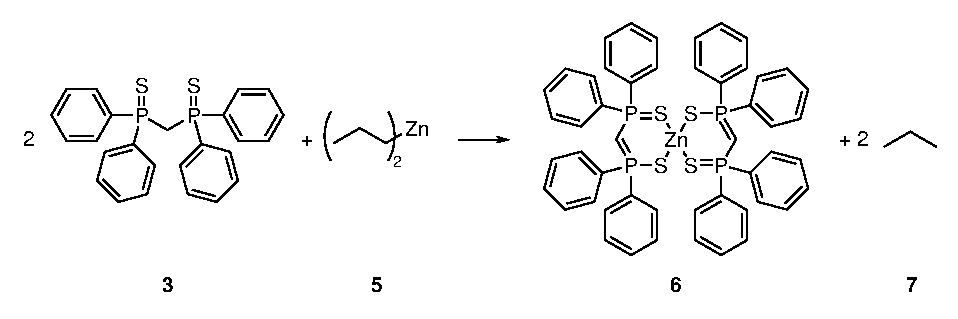
\includegraphics[width=5.5cm]{Komplex.eps},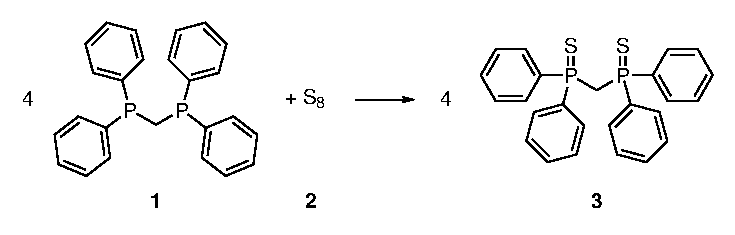
\includegraphics[width=5.5cm]{Ligand.eps}}

% Kastenarray mit 4 Kästen, 2.5 cm breit, 3 cm hoch, Abstand 0.2 cm und tight=f,
% da danach noch ein Kastenarray folgt.
\kastenarray[2.5cm]{3cm}[0.2cm][]{G,J,I,W}{1234,6425,672,6489}

% Kastenarray mit 3 Kästen, 3 cm breit, 4 cm hoch, Abstand 0cm und tight leer gelassen,
% da danach Text folgt.
\kastenarray[3cm]{4cm}[0cm][]{C,D,S}{0123,4567,890a}

% Kastenarray mit 3 Kästen, Breite automatisch bestimmt, 2 cm hoch, Abstand 0cm und 
% tight leer gelassen, da danach Text folgt.
\kastenarray{2cm}[0cm][f]{C,D,S}{0123,4567,890a}


% kastenarraycustom malt Kästen ohne Labels. 
% Und ihre Inhalte sind nicht von opt{} abhängig.
\kastenarraycustom{2cm}[0cm][]{11, 22, 33, 44}

Hier ein Text.


% Noch zwei Kastenarrays.
\kastenarray[7cm]{7cm}{1,2}{Molekuel1,Molekuel2}

\kastenarray[7cm]{7cm}[0cm][]{3,4}{Molekuel3,Molekuel4}

Hier ein Text. \newpage \aufgabenende
\end{document}
